% ============================================================
% 第10章：数列极限的直观——趋近一个数的感觉
% ============================================================

\chapter{数列极限的直观——趋近一个数的感觉}

\begin{applicationbox}
\textbf{学完本章你能做什么？}
\begin{enumerate}
  \item 建立数列极限的\textbf{直观概念}——什么是"趋近"？
  \item 区分\textbf{收敛数列}（有极限）和\textbf{发散数列}（没有极限）
  \item 理解极限的"\textbf{ε 带}"几何意义——为下一章的严格定义做准备
\end{enumerate}
\end{applicationbox}


% ============================================================
\section{从第9章来——数列的项在"变化"}
% ============================================================

第9章我们学了数列——\(a_1, a_2, a_3, \ldots, a_n, \ldots\)

当 \(n\) 越来越大时，数列的项会怎么变化？

\begin{center}
\begin{tabular}{c|c|c}
\textbf{数列} & \textbf{当 \(n\) 很大时的行为} & \textbf{结论} \\
\hline
\(a_n = 1/n\) & 越来越接近 0 & \textbf{收敛}到 0 \\
\(a_n = n/(n+1)\) & 越来越接近 1 & \textbf{收敛}到 1 \\
\(a_n = 2^n\) & 越来越大，没有上限 & \textbf{发散}到无穷大 \\
\(a_n = (-1)^n\) & 在 -1 和 1 之间来回跳 & \textbf{发散}（振荡） \\
\end{tabular}
\end{center}

\textbf{极限}研究的就是：当 \(n\) 无限增大时，数列趋近于什么？


% ============================================================
\section{极限的直观概念}
% ============================================================

\begin{definitionbox}[极限的直观定义]
如果当 \(n\) 越来越大时，\(a_n\) 无限趋近于一个固定的数 \(L\)，
那么称 \(L\) 是数列 \(\{a_n\}\) 的\textbf{极限}（读作 jí xiàn，英文 limit）。

记作：
\[
\lim_{n \to \infty} a_n = L
\]

读作："当 \(n\) 趋向于无穷大时，\(a_n\) 的极限等于 \(L\)"。
\end{definitionbox}

\begin{examplebox}[1——从数字中感受极限]
数列 \(a_n = 1/n\)：

\[
a_1 = 1,\; a_2 = 0.5,\; a_3 \approx 0.333,\; a_4 = 0.25,\; a_5 = 0.2
\]
\[
a_{10} = 0.1,\; a_{100} = 0.01,\; a_{1000} = 0.001,\; a_{10000} = 0.0001
\]

\textbf{感受：} \(n\) 每扩大 10 倍，\(a_n\) 缩小到原来的 1/10。\\
当 \(n\) 无限大时，\(a_n\) 无限接近 0——所以 \(\lim_{n \to \infty} \dfrac{1}{n} = 0\)。
\end{examplebox}


% ============================================================
\section{收敛数列——有极限}
% ============================================================

\begin{examplebox}[2——收敛的例子]
\begin{center}
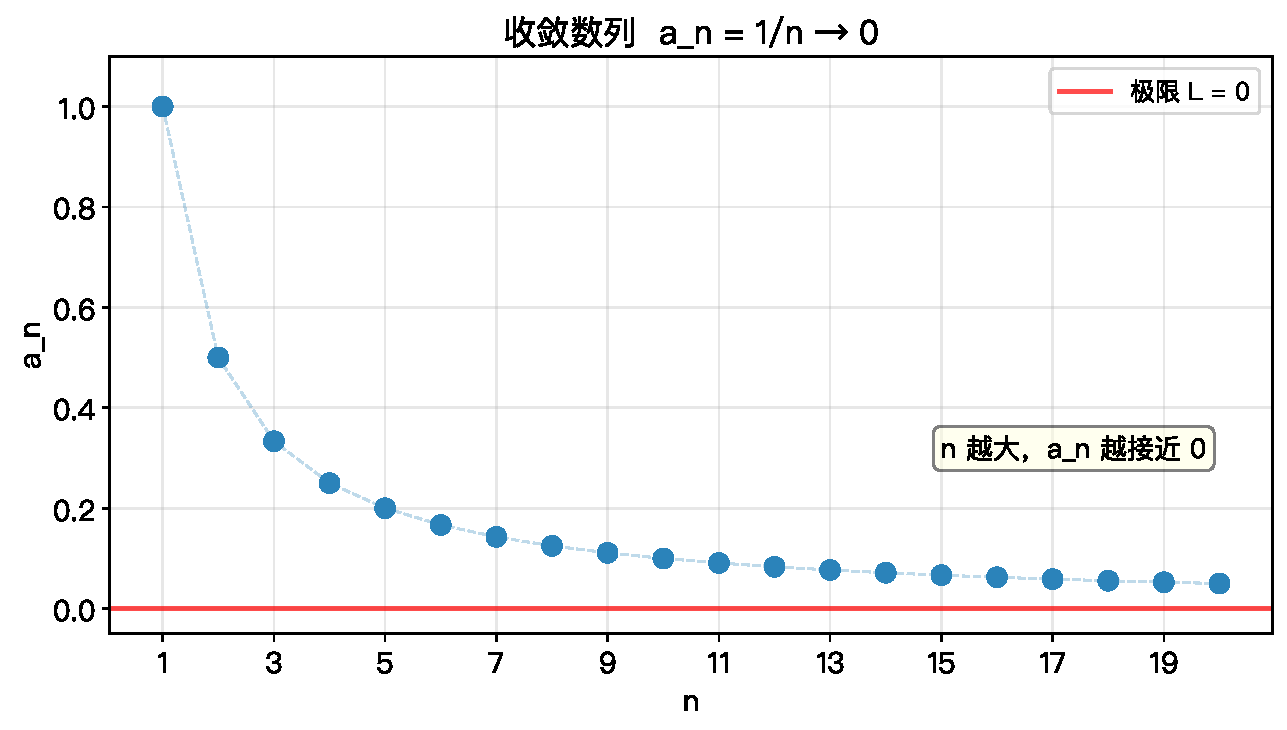
\includegraphics[width=0.85\textwidth]{figures/ch10_convergent.pdf}
\end{center}

数列 \(a_n = \dfrac{1}{n}\)：
\begin{itemize}
  \item 从 1 开始，逐渐下降
  \item 越来越接近 0，但永远不等于 0
  \item \(\displaystyle \lim_{n \to \infty} \frac{1}{n} = 0\)
\end{itemize}
\end{examplebox}

\begin{examplebox}[3——更多收敛数列]
\[
(1)\; a_n = \frac{n}{n+1}：\quad a_1=\frac12,\; a_2=\frac23,\; a_3=\frac34,\; \ldots \to 1
\]
\[
(2)\; a_n = \frac{1}{2^n}：\quad a_1=\frac12,\; a_2=\frac14,\; a_3=\frac18,\; \ldots \to 0
\]
\[
(3)\; a_n = \frac{1}{n^2}：\quad a_1=1,\; a_2=\frac14,\; a_3=\frac19,\; \ldots \to 0
\]

\textbf{验证 \(\lim_{n \to \infty} \dfrac{n}{n+1} = 1\)：}
\[
n=10: \frac{10}{11} \approx 0.909,\quad
n=100: \frac{100}{101} \approx 0.990,\quad
n=1000: \frac{1000}{1001} \approx 0.999
\]
确实越来越接近 1。
\end{examplebox}


% ============================================================
\section{发散数列——没有极限}
% ============================================================

不是所有数列都有极限。有三种常见的发散情况。

\subsection{趋于无穷}

\begin{examplebox}[4——发散到无穷大]
\begin{center}
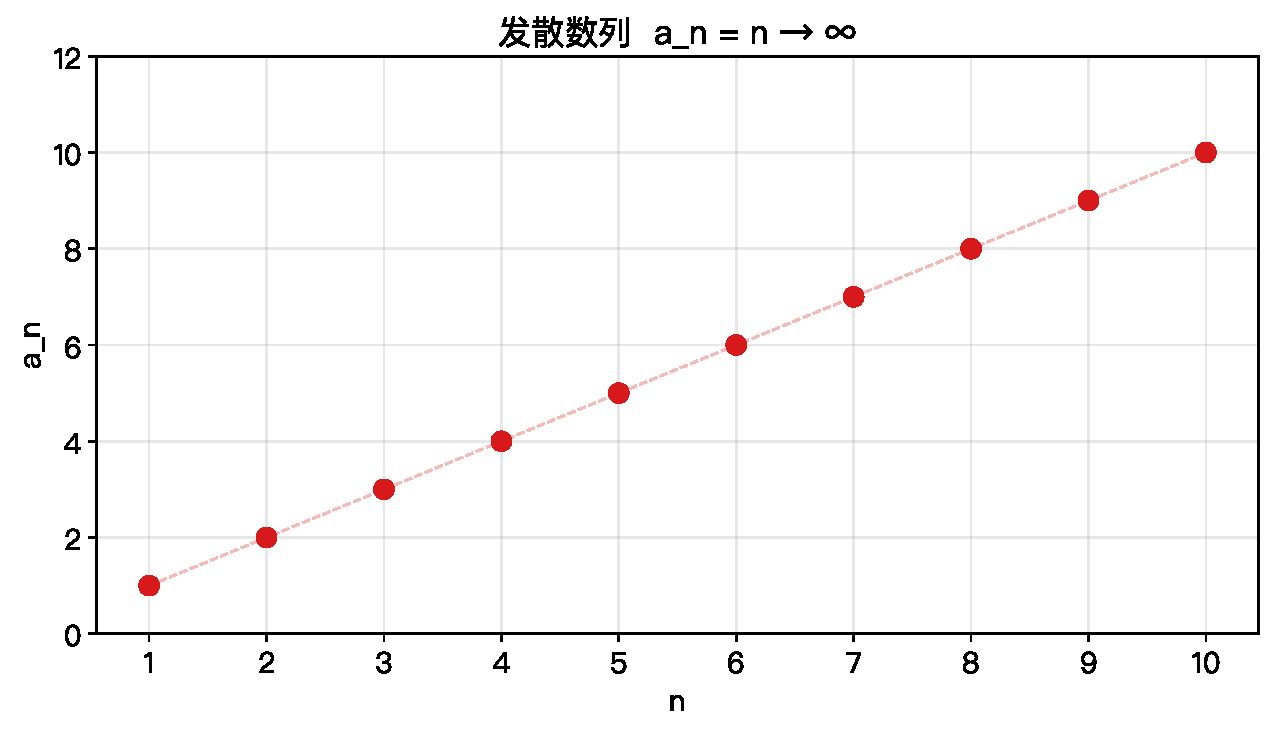
\includegraphics[width=0.85\textwidth]{figures/ch10_divergent.pdf}
\end{center}

数列 \(a_n = n\)：\(1, 2, 3, 4, \ldots\)——越来越大，没有上限。

这时我们说"极限不存在"或"发散到无穷大"。

有时也记作 \(\displaystyle \lim_{n \to \infty} n = \infty\)，但这只是一种记号，\textbf{不是真正的极限}（因为无穷大不是一个数）。
\end{examplebox}

\subsection{振荡发散}

\begin{examplebox}[5——振荡发散]
\begin{center}
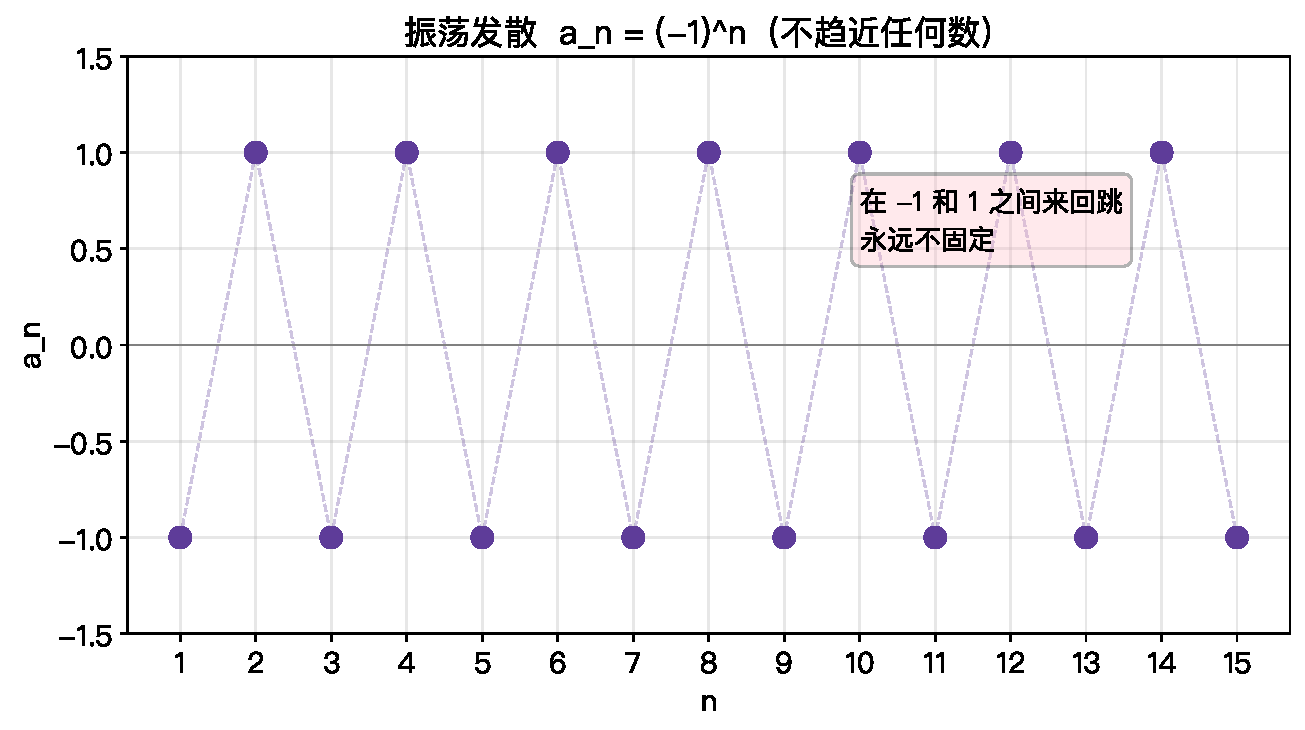
\includegraphics[width=0.85\textwidth]{figures/ch10_oscillating_divergent.pdf}
\end{center}

数列 \(a_n = (-1)^n\)：\(-1, 1, -1, 1, -1, 1, \ldots\)

它既不趋近任何数，也不趋于无穷——它在两个值之间来回跳。\\
这种发散叫\textbf{振荡发散}。
\end{examplebox}


% ============================================================
\section{极限的"ε带"几何意义}
% ============================================================

收敛数列的核心特征是：\textbf{从某项之后，所有项都"挤"在极限附近的一个小范围内}。

\begin{examplebox}[6——ε带的直观理解]
\begin{center}
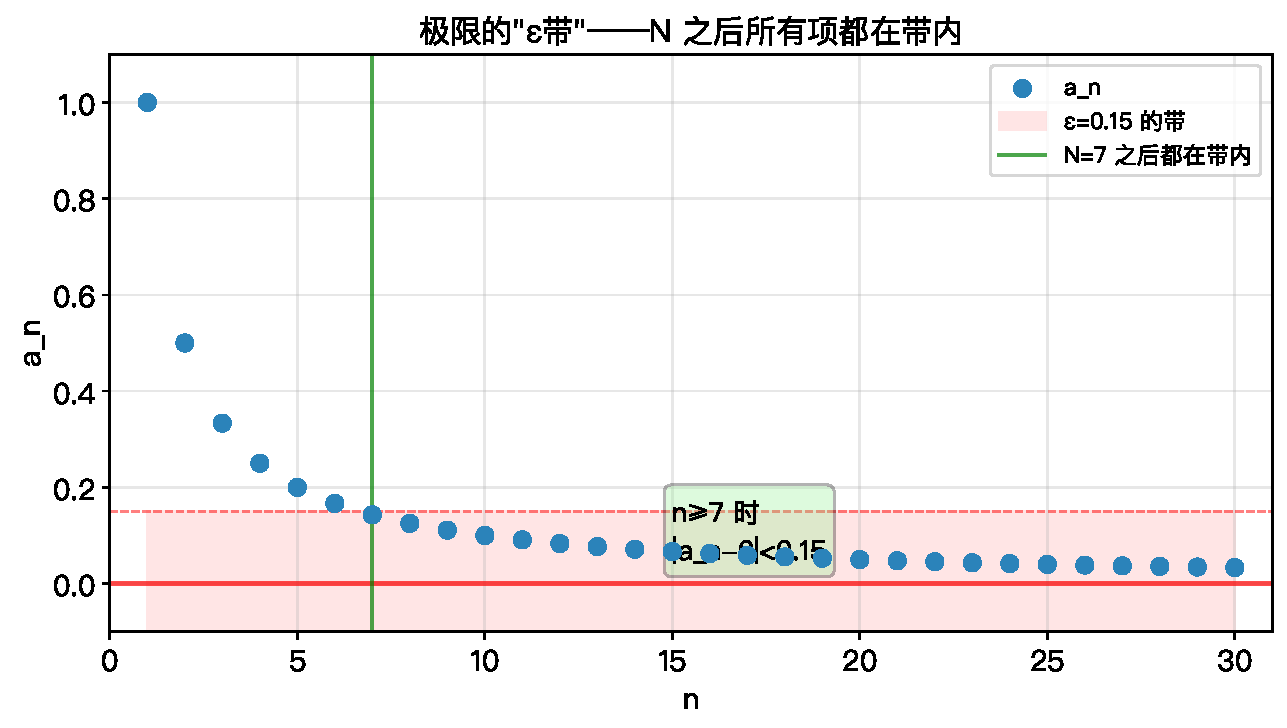
\includegraphics[width=0.85\textwidth]{figures/ch10_epsilon_band.pdf}
\end{center}

取一个很小的正数 \(\varepsilon\)（读作"伊普西龙"），在极限 \(L=0\) 周围画一条宽为 \(2\varepsilon\) 的带：
\begin{itemize}
  \item 红色带：\(|a_n - 0| < \varepsilon\) 的范围
  \item 从 \(n \ge 7\) 开始，所有项都落在这个带内
  \item \(n\) 越大，带可以取得越窄，但总存在一个 \(N\) 让之后的项都在带内
\end{itemize}

这就是\textbf{极限的核心思想}：不管你把带子取得多窄（多小的 \(\varepsilon\)），
总能找到一项 \(N\)，使得 \(N\) 之后的所有项都在带子里。
\end{examplebox}


% ============================================================
\section{常见极限的直观判断}
% ============================================================

\begin{examplebox}[7——几个重要极限]
\[
(1)\; \lim_{n \to \infty} \frac{1}{n^p} = 0 \quad (p > 0)
\]
\[
(2)\; \lim_{n \to \infty} q^n = 0 \quad (|q| < 1)
\]
\[
(3)\; \lim_{n \to \infty} \sqrt[n]{a} = 1 \quad (a > 0)
\]

\textbf{验证：}
\[
\frac{1}{\sqrt{n}} \to 0：\; \frac{1}{\sqrt{100}} = 0.1,\; \frac{1}{\sqrt{10000}} = 0.01
\]
\[
\left(\frac{1}{2}\right)^n \to 0：\; \left(\frac{1}{2}\right)^{10} = \frac{1}{1024} \approx 0.001
\]
\[
\sqrt[n]{2} \to 1：\; \sqrt[10]{2} \approx 1.072,\; \sqrt[100]{2} \approx 1.007
\]
\end{examplebox}


% ============================================================
\section{符号卡片}
% ============================================================

\begin{symbolcard}
\(\displaystyle \lim_{n \to \infty}\) & \verb|\lim_{n\to\infty}| & 读作"当 n 趋向无穷时的极限" & 极限符号 \\
\(\varepsilon\) & \verb|\varepsilon| & 读作"伊普西龙" & 任意小的正数 \\
\(a_n \to L\) & \verb|a_n \to L| & 读作"a n 趋近于 L" & 数列收敛到 L \\
发散 & —— & 读作"fā sàn" & 没有极限 \\
\end{symbolcard}


% ============================================================
\section{本章小结}
% ============================================================

\begin{progressbox}
\textbf{极限的直观}：\(n\) 越大，\(a_n\) 越接近 \(L\)

\textbf{收敛}：有极限（如 \(\dfrac{1}{n} \to 0\)，\(\dfrac{n}{n+1} \to 1\)）

\textbf{发散}：没有极限——可能趋于无穷，可能振荡

\textbf{ε带思想}：对任意 \(\varepsilon > 0\)，存在 \(N\) 使 \(n \ge N\) 时 \(|a_n - L| < \varepsilon\)

\textbf{重要极限}：\(\dfrac{1}{n^p} \to 0\)（\(p>0\)），\(q^n \to 0\)（\(|q|<1\)），\(\sqrt[n]{a} \to 1\)（\(a>0\)）
\end{progressbox}

\subsection*{通往下一章}

\textbf{这一章}你从直观上理解了"极限"是什么——数列趋近于一个数。

\textbf{下一章}将是数学分析中\textbf{第一次真正严格的定义}：
用 ε-N 语言精确地定义极限。准备好了吗？


% ============================================================
% 习题
% ============================================================
\section{习题}

% ===== 送分 =====

\begin{exercise}[0]
写出 \(\displaystyle\lim_{n\to\infty} \frac{1}{n}\) 的值。
\end{exercise}

\begin{exercise}[0]
判断：数列 \(a_n = n\) 是收敛还是发散？
\end{exercise}

\begin{exercise}[0]
判断：数列 \(a_n = (-1)^n\) 是收敛还是发散？
\end{exercise}

\begin{exercise}[0]
如果 \(\displaystyle\lim_{n\to\infty} a_n = 5\)，当 \(n\) 很大时，\(a_n\) 接近多少？
\end{exercise}

% ===== 简单 =====

\begin{exercise}[1]
计算 \(a_n = \dfrac{n}{n+1}\) 在 \(n=1, 10, 100, 1000\) 时的值，并猜测极限。
\end{exercise}

\begin{exercise}[1]
判断以下数列是否收敛（若收敛，极限是多少）：
\[
(1)\; a_n = \frac{1}{n^2} \qquad
(2)\; a_n = 3 + \frac{1}{n} \qquad
(3)\; a_n = (-1)^n n
\]
\end{exercise}

\begin{exercise}[1]
已知 \(\displaystyle\lim_{n\to\infty} a_n = 2\)，当 \(n\) 很大时，\(1 + a_n\) 接近多少？
\end{exercise}

\begin{exercise}[1]
填空：若 \(|q| < 1\)，则 \(\displaystyle\lim_{n\to\infty} q^n = \_\_\_\_\)。
\end{exercise}

% ===== 基础 =====

\begin{exercise}[2]
求极限（利用已知结论）：
\[
(1)\; \lim_{n\to\infty} \frac{1}{\sqrt{n}} \qquad
(2)\; \lim_{n\to\infty} \left(\frac{2}{3}\right)^n \qquad
(3)\; \lim_{n\to\infty} \frac{n}{2n+1}
\]
\end{exercise}

\begin{exercise}[2]
写出一个收敛到 3 的数列（至少写出通项公式）。
\end{exercise}

\begin{exercise}[2]
举例说明：一个数列可以有界但不收敛。
\end{exercise}

\begin{exercise}[2]
已知 \(a_n = \dfrac{2n+1}{n}\)，求 \(\displaystyle\lim_{n\to\infty} a_n\)。
\end{exercise}

% ===== 普通 =====

\begin{exercise}[3]
求极限：
\[
(1)\; \lim_{n\to\infty} \frac{3n^2 + 2}{n^2 + 1} \qquad
(2)\; \lim_{n\to\infty} \frac{n + 1}{n^2 + 2}
\]
（提示：分子分母同除以最高次项）
\end{exercise}

\begin{exercise}[3]
已知 \(a_n = \dfrac{1}{2^n}\)，求满足 \(|a_n - 0| < 0.001\) 的最小 \(n\)。
\end{exercise}

\begin{exercise}[3]
证明：数列 \(a_n = \dfrac{1}{n}\) 是递减且有下界的。
\end{exercise}

\begin{exercise}[3]
观察数列 \(a_n = \sqrt{n+1} - \sqrt{n}\) 的前几项，猜猜极限是多少？
（提示：有理化 \( \sqrt{n+1} - \sqrt{n} = \dfrac{1}{\sqrt{n+1} + \sqrt{n}} \)）
\end{exercise}

\begin{exercise}[3]
数列 \(a_n = 0.333\ldots 3\)（\(n\) 个 3）的极限是多少？
\end{exercise}

% ===== 中等 =====

\begin{exercise}[4]
用极限的 ε 带思想解释：为什么 \(\displaystyle\lim_{n\to\infty} \frac{1}{n^2} = 0\)？
取 \(\varepsilon = 0.01\)，找到对应的 \(N\)。
\end{exercise}

\begin{exercise}[4]
若 \(\displaystyle\lim_{n\to\infty} a_n = 3\)，证明 \(\displaystyle\lim_{n\to\infty} (2a_n - 1) = 5\)。
\end{exercise}

\begin{exercise}[4]
求极限：
\[
\lim_{n\to\infty} \left(\frac{1}{n} + \frac{2}{n} + \frac{3}{n} + \cdots + \frac{n}{n}\right) \frac{1}{n}
\]
（提示：先求和，再取极限）
\end{exercise}

\begin{exercise}[4]
已知数列 \(a_n = \dfrac{n}{2^n}\)，计算前几项，猜测极限。
（提示：\(2^n\) 的增长比 \(n\) 快得多）
\end{exercise}

\begin{exercise}[4]
判断：若 \(a_n\) 收敛，则 \(a_n\) 一定有界。这个说法对吗？为什么？
\end{exercise}

% ===== 进阶 =====

\begin{exercise}[5]
已知 \(a_n = \dfrac{n^2 + n + 1}{3n^2 - 2n + 4}\)，求 \(\displaystyle\lim_{n\to\infty} a_n\)。
\end{exercise}

\begin{exercise}[5]
构造一个数列，它不收敛、不趋于无穷、也不是振荡发散（提示：考虑 \(a_n = \sin n\)）。
\end{exercise}

\begin{exercise}[5]
若 \(a_n \to 0\)，\(b_n\) 有界，证明 \(a_n b_n \to 0\)。
\end{exercise}

\begin{exercise}[5]
证明：若 \(\displaystyle\lim_{n\to\infty} a_n = L\)，则 \(\displaystyle\lim_{n\to\infty} |a_n| = |L|\)。
（提示：利用 \(||a_n| - |L|| \le |a_n - L|\)）
\end{exercise}

% ===== 拔高 =====

\begin{exercise}[6]
数列 \(a_n = \left(1 + \dfrac{1}{n}\right)^n\) 是单调递增且有上界的。
\begin{enumerate}
  \item[(1)] 计算 \(a_1, a_2, a_5, a_{10}, a_{100}\)（用计算器或代码）
  \item[(2)] 这个数列的极限是一个著名的常数——是多少？
\end{enumerate}
\end{exercise}

\begin{exercise}[6]
设 \(a_n = \dfrac{1 \times 3 \times 5 \times \cdots \times (2n-1)}{2 \times 4 \times 6 \times \cdots \times (2n)}\)。
\begin{enumerate}
  \item[(1)] 计算 \(a_1, a_2, a_3, a_4\)
  \item[(2)] 证明 \(a_n\) 递减且有下界
  \item[(3)] 猜猜极限是多少？
\end{enumerate}
\end{exercise}

\begin{exercise}[6]
已知 \(a_1 = 1\)，\(a_{n+1} = \dfrac{1}{2}\left(a_n + \dfrac{2}{a_n}\right)\)。
\begin{enumerate}
  \item[(1)] 计算 \(a_2, a_3, a_4, a_5\)（保留小数）
  \item[(2)] 猜猜极限——它逼近什么数？
\end{enumerate}
\end{exercise}

% ===== 极难 =====

\begin{exercise}[7]
设 \(a_1 = 1\)，\(a_{n+1} = \dfrac{a_n + 2}{a_n + 1}\)。
\begin{enumerate}
  \item[(1)] 证明 \(1 \le a_n \le 2\) 对所有 \(n\) 成立
  \item[(2)] 证明 \(\{a_n\}\) 是单调的（递增还是递减？）
  \item[(3)] 求 \(\displaystyle\lim_{n\to\infty} a_n\)（提示：设极限为 \(L\)，在递推式两边取极限）
\end{enumerate}

\textbf{说明：} 这道题展示了求极限的重要方法——
先证单调有界（保证极限存在），再在递推式中取极限解出 \(L\)。
这是数学分析中最经典的方法之一。
\end{exercise}
